% ---------------------------------------------------------------------------
% main.tex — Caderno 1: Por que planejar experimentos.
% Primeiro dos cinco cadernos de Planejamento de Experimentos (DoE) escritos
% para a disciplina do IME. Compilação:
%   $env:PATH = "C:\Users\Narcísius\AppData\Local\Programs\MiKTeX\miktex\bin\x64;" + $env:PATH
%   pdflatex -interaction=nonstopmode main.tex   (três vezes, por causa do sumário)
% ---------------------------------------------------------------------------
\documentclass{doeapostila}

% ---------------------------------------------------------------------------
% macros.tex — notação matemática comum aos cinco cadernos.
% Fixada antes de qualquer caderno começar, para os cinco não divergirem.
% Uso: % ---------------------------------------------------------------------------
% macros.tex — notação matemática comum aos cinco cadernos.
% Fixada antes de qualquer caderno começar, para os cinco não divergirem.
% Uso: % ---------------------------------------------------------------------------
% macros.tex — notação matemática comum aos cinco cadernos.
% Fixada antes de qualquer caderno começar, para os cinco não divergirem.
% Uso: \input{../estilo/macros} no preâmbulo de cada main.tex.
% ---------------------------------------------------------------------------

% Somas de quadrados
\newcommand{\SQT}{\mathrm{SQ}_{\mathrm{T}}}    % total
\newcommand{\SQR}{\mathrm{SQ}_{\mathrm{R}}}    % da regressão
\newcommand{\SQr}{\mathrm{SQ}_{\mathrm{r}}}    % residual
\newcommand{\SQfaj}{\mathrm{SQ}_{\mathrm{faj}}}% falta de ajuste
\newcommand{\SQep}{\mathrm{SQ}_{\mathrm{ep}}}  % erro puro

% Médias quadráticas: \MQ{R}, \MQ{r}, \MQ{faj}, \MQ{ep}
\newcommand{\MQ}[1]{\mathrm{MQ}_{\mathrm{#1}}}

% Coeficientes de determinação
\newcommand{\Rdois}{R^{2}}
\newcommand{\Rajus}{R^{2}_{\mathrm{aj}}}

% Efeitos: \efeito{1}, \efeito{12}
\newcommand{\efeito}[1]{E_{#1}}

% Álgebra matricial do ajuste por mínimos quadrados
\newcommand{\vetbeta}{\boldsymbol{\beta}}
\newcommand{\matX}{\mathbf{X}}
\newcommand{\vety}{\mathbf{y}}
 no preâmbulo de cada main.tex.
% ---------------------------------------------------------------------------

% Somas de quadrados
\newcommand{\SQT}{\mathrm{SQ}_{\mathrm{T}}}    % total
\newcommand{\SQR}{\mathrm{SQ}_{\mathrm{R}}}    % da regressão
\newcommand{\SQr}{\mathrm{SQ}_{\mathrm{r}}}    % residual
\newcommand{\SQfaj}{\mathrm{SQ}_{\mathrm{faj}}}% falta de ajuste
\newcommand{\SQep}{\mathrm{SQ}_{\mathrm{ep}}}  % erro puro

% Médias quadráticas: \MQ{R}, \MQ{r}, \MQ{faj}, \MQ{ep}
\newcommand{\MQ}[1]{\mathrm{MQ}_{\mathrm{#1}}}

% Coeficientes de determinação
\newcommand{\Rdois}{R^{2}}
\newcommand{\Rajus}{R^{2}_{\mathrm{aj}}}

% Efeitos: \efeito{1}, \efeito{12}
\newcommand{\efeito}[1]{E_{#1}}

% Álgebra matricial do ajuste por mínimos quadrados
\newcommand{\vetbeta}{\boldsymbol{\beta}}
\newcommand{\matX}{\mathbf{X}}
\newcommand{\vety}{\mathbf{y}}
 no preâmbulo de cada main.tex.
% ---------------------------------------------------------------------------

% Somas de quadrados
\newcommand{\SQT}{\mathrm{SQ}_{\mathrm{T}}}    % total
\newcommand{\SQR}{\mathrm{SQ}_{\mathrm{R}}}    % da regressão
\newcommand{\SQr}{\mathrm{SQ}_{\mathrm{r}}}    % residual
\newcommand{\SQfaj}{\mathrm{SQ}_{\mathrm{faj}}}% falta de ajuste
\newcommand{\SQep}{\mathrm{SQ}_{\mathrm{ep}}}  % erro puro

% Médias quadráticas: \MQ{R}, \MQ{r}, \MQ{faj}, \MQ{ep}
\newcommand{\MQ}[1]{\mathrm{MQ}_{\mathrm{#1}}}

% Coeficientes de determinação
\newcommand{\Rdois}{R^{2}}
\newcommand{\Rajus}{R^{2}_{\mathrm{aj}}}

% Efeitos: \efeito{1}, \efeito{12}
\newcommand{\efeito}[1]{E_{#1}}

% Álgebra matricial do ajuste por mínimos quadrados
\newcommand{\vetbeta}{\boldsymbol{\beta}}
\newcommand{\matX}{\mathbf{X}}
\newcommand{\vety}{\mathbf{y}}


\definecaderno{1}{Por que planejar experimentos}

\begin{document}

\begin{center}
  {\LARGE\bfseries Caderno 1}\par\smallskip
  {\Large Por que planejar experimentos}\par\smallskip
  {\normalsize Murilo Miguel Narciso}\par\smallskip
  {\footnotesize Programa de Planejamento de Experimentos \textbullet{} Instituto Militar de Engenharia}
\end{center}

\vspace{0.6\baselineskip}

\noindent
Este é o primeiro de cinco cadernos preparados para a disciplina de
Planejamento de Experimentos ministrada no Instituto Militar de Engenharia.
Os exemplos combinam casos clássicos da literatura de planejamento com
situações reais do trabalho experimental do autor, que investiga compósitos
de solo, fibra e cimento empregando fibra vegetal de origem amazônica. Essa
combinação é deliberada: os princípios se sustentam nos dois contextos, e o
segundo mostra que eles não são um exercício de sala, mas uma resposta a
restrições concretas de laboratório.

\vspace{0.6\baselineskip}

\tableofcontents

\section{Introdução}
\label{sec:introducao}

A distância entre a sala de aula e a bancada de laboratório aparece assim
que um experimento real precisa ser conduzido. Na teoria, um efeito existe
ou não existe, e a comparação entre duas condições produz uma diferença
limpa. No laboratório, toda medição carrega variação que nada tem a ver com
a pergunta feita: a balança oscila, o corpo de prova não é perfeitamente
homogêneo, a temperatura da sala muda entre a manhã e a tarde. Ignorar essa
variação leva a conclusões que não resistem a uma segunda tentativa;
respeitá-la exige um método, e é esse método que este caderno introduz.

Antes de qualquer ensaio ser executado, quatro perguntas precisam de
resposta. Quais ensaios devem ser realizados, dentre todas as combinações
possíveis das variáveis de interesse. Quantas réplicas cada condição exige,
para que a variação natural do processo não seja confundida com um efeito
real. Quais variáveis devem ser deliberadamente alteradas ao longo do
experimento, e quais devem ser mantidas fixas ou apenas registradas. Em
quantos níveis cada uma dessas variáveis será testada. Essas quatro
perguntas formam o roteiro do planejamento de experimentos, e cada uma delas
é retomada em algum ponto deste caderno.

Essas quatro perguntas não são um exercício isolado da prática posterior de
um pesquisador. A forma como um experimento foi planejado determina o que
pode ser afirmado depois dele, e um leitor experiente de artigo científico
procura, na seção de materiais e métodos, exatamente as respostas a essas
quatro perguntas antes de aceitar qualquer conclusão apresentada nos
resultados. Um estudo que varia um fator de cada vez, sem réplica declarada
e sem menção à ordem de execução, carrega uma fragilidade que nenhuma
análise estatística posterior consegue disfarçar. O Caderno~5 retoma esse
ponto ao final da série e mostra, em detalhe, o que declarar num artigo
para que essa fragilidade não exista.

O caderno segue uma ordem específica. As Seções~\ref{sec:fator-nivel} a
\ref{sec:ofat} estabelecem o vocabulário e mostram por que a alternativa mais
intuitiva, variar um fator de cada vez, falha justamente quando os fatores
interagem. As Seções~\ref{sec:erros-medida} e \ref{sec:erro-laboratorio}
tratam da origem do erro experimental, primeiro em termos gerais e depois no
contexto concreto do laboratório de materiais. As Seções~\ref{sec:replicas}
a \ref{sec:blocagem} apresentam as três ferramentas que o planejamento de
experimentos oferece contra esse erro: réplica, aleatorização e blocagem. A
Seção~\ref{sec:material-escasso} discute o que acontece quando o número de
ensaios não é uma escolha livre, mas uma restrição imposta pela quantidade
de material disponível, e a Seção~\ref{sec:exemplo-final} fecha o caderno
aplicando tudo isso ao planejamento de um estudo real.

\section{Fator, nível e resposta}
\label{sec:fator-nivel}

Um experimento planejado distingue três categorias de variável. O fator é
uma entrada que o experimentador escolhe deliberadamente alterar. O nível é
um dos valores específicos atribuídos a um fator dentro do experimento. A
resposta é a grandeza de saída medida, aquela cujo comportamento se deseja
explicar ou otimizar.

Fatores se dividem em quantitativos e qualitativos. Um fator quantitativo
assume valores numéricos ao longo de uma escala contínua, como a temperatura
de uma reação ou o teor de cimento de uma mistura, e admite níveis
intermediários entre os extremos testados. Um fator qualitativo assume
categorias sem ordenação numérica natural, como o tipo de catalisador
empregado ou a procedência de um lote de matéria-prima, e não faz sentido
falar em um nível intermediário entre duas categorias. Essa distinção
importa porque apenas fatores quantitativos permitem ajustar um modelo de
superfície de resposta e prever o comportamento em pontos não ensaiados,
assunto do Caderno~4.

É útil também pensar no experimento como um sistema com entradas e saída. As
entradas controláveis são os fatores propriamente ditos, escolhidos e
fixados pelo experimentador em cada ensaio. As entradas não controláveis, ou
ruídos, variam por conta própria, como a umidade do ar num dia de ensaio, e
não podem ser fixadas, mas seus efeitos podem ser neutralizados por
aleatorização e blocagem, temas das Seções~\ref{sec:aleatorizacao} e
\ref{sec:blocagem}. A resposta é o que se observa na saída desse sistema, e
sua escolha precisa antecipar a pergunta de pesquisa: medir uma grandeza que
não se relaciona com a hipótese em jogo invalida o experimento antes mesmo
de ele começar.

A fronteira entre entrada controlável e ruído não é uma propriedade
intrínseca da variável, mas uma decisão de projeto do experimento. A
umidade do ar de um laboratório é ruído quando o experimentador não dispõe
de câmara climatizada e apenas registra seu valor a cada ensaio; a mesma
grandeza torna-se fator controlável assim que uma câmara desse tipo está
disponível e a umidade passa a ser fixada deliberadamente em níveis
escolhidos. Reconhecer corretamente essa fronteira, para os recursos
efetivamente disponíveis, evita duas armadilhas simétricas: tratar como
fixo algo que na verdade varia sem ser registrado, o que contamina a
resposta com uma fonte de erro não identificada, e tentar controlar
formalmente uma variável que os recursos do laboratório não permitem
manter estável na prática, o que produz uma matriz de ensaios que a
bancada não consegue honrar.

\begin{aplicacao}{Fatores, níveis e resposta num experimento de rendimento}
  Um experimento clássico de engenharia química investiga o rendimento de
  uma reação em função da temperatura e do catalisador empregado. A
  Tabela~\ref{tab:fatores-catalisador} apresenta o planejamento fatorial
  completo com dois fatores em dois níveis, conduzido com duas réplicas por
  condição.

  \begin{table}[H]
    \centering
    \caption{Planejamento fatorial $2^{2}$ de um experimento de rendimento
      de reação. A temperatura é fator quantitativo e o catalisador é fator
      qualitativo; a resposta é o rendimento, em \%.}
    \label{tab:fatores-catalisador}
    \begin{tabular}{c S[table-format=3.0] c S[table-format=2.0] S[table-format=2.0] S[table-format=2.0]}
      \toprule
      {Ensaio} & {T (\si{\kelvin})} & {Catalisador} & {Réplica 1} & {Réplica 2} & {Média} \\
      \midrule
      1 & 313 & A & 57 & 61 & 59 \\
      2 & 333 & A & 92 & 88 & 90 \\
      3 & 313 & B & 55 & 53 & 54 \\
      4 & 333 & B & 66 & 70 & 68 \\
      \bottomrule
    \end{tabular}
  \end{table}

  A temperatura assume os níveis \qty{313}{\kelvin} e \qty{333}{\kelvin}, um
  intervalo contínuo do qual esses dois valores são apenas os extremos
  escolhidos, o que caracteriza um fator quantitativo. O catalisador assume
  os rótulos A e B, sem escala numérica entre eles, o que caracteriza um
  fator qualitativo. A resposta, o rendimento em \%, foi escolhida por ser a
  grandeza que a pergunta de pesquisa original visava explicar. Este mesmo
  conjunto de dados é retomado nas Seções~\ref{sec:replicas} e, com maior
  profundidade, no Caderno~2 (fonte: Peixoto, Capítulo 3, páginas 2 a 9).
\end{aplicacao}

\section{A hipótese de pesquisa como pré-condição}
\label{sec:hipotese}

O planejamento de experimentos organiza a coleta de dados, mas não substitui
a etapa anterior a ele: a formulação de uma hipótese de pesquisa apoiada em
revisão bibliográfica. É a hipótese que indica quais fatores provavelmente
influenciam a resposta, qual forma funcional é esperada entre eles, e qual
faixa de níveis é fisicamente razoável testar. Sem essa etapa prévia, o
experimentador corre dois riscos simétricos: variar fatores irrelevantes,
desperdiçando ensaios sobre algo que a teoria já descartaria, ou deixar de
lado um fator que a literatura já indicava como determinante.

A revisão bibliográfica também define a forma esperada da relação entre
fator e resposta antes que qualquer dado seja coletado. Isso é decisivo
porque a mesma tabela de ensaios pode ser lida à luz de modelos distintos, e
o modelo certo é aquele sustentado pela teoria do fenômeno, não aquele que
parecer ajustar melhor depois do fato. Um ajuste de altíssima qualidade
obtido com um modelo sem respaldo teórico é, na melhor das hipóteses,
coincidência, e o Caderno~3 volta a esse ponto ao discutir os limites do
coeficiente de determinação.

\begin{aplicacao}{A hipótese que precede o planejamento}
  A velocidade de queima de uma pólvora, $v$, em função da pressão de
  operação, $P$, é objeto de uma hipótese estabelecida pela teoria da
  combustão antes de qualquer ensaio: espera-se uma relação de potência da
  forma $v = k \cdot P^{a}$. Essa hipótese, e não uma inspeção posterior dos
  dados, é que orienta o planejamento: dezoito níveis de pressão foram
  varridos de \qty{1}{psi} a \qty{69}{psi}, e a relação foi linearizada por
  logaritmo, $\log_{10} v = \log_{10} k + a \log_{10} P$, para ser tratada
  por regressão linear simples. O ajuste aos dezoito pontos produziu
  $a = \num{0.391856}$ e $\log_{10} k = \num{0.592346}$, com
  $\Rdois = \num{0.999587}$, resultado coerente com a hipótese de partida.
  O ponto didático não é o valor alto de $\Rdois$, mas o fato de que ele só
  é interpretável porque a forma do modelo foi fixada antes da coleta, e não
  escolhida depois para maximizar o ajuste (fonte: Peixoto, Capítulo 5,
  páginas 21 e 22).
\end{aplicacao}

\section{Por que variar um fator de cada vez não funciona}
\label{sec:ofat}

A alternativa mais intuitiva ao planejamento fatorial é variar um fator de
cada vez, mantendo os demais fixos, e mover cada um deles até que sua
resposta pare de melhorar. Esse procedimento tem uma falha estrutural
quando os fatores interagem, isto é, quando o efeito de um fator sobre a
resposta depende do nível em que o outro fator se encontra. Nesses casos, a
busca sequencial estaciona num ponto que é ótimo apenas em relação aos
cortes unidimensionais percorridos, e não em relação à superfície completa.

A Figura~\ref{fig:ofat} apresenta uma superfície de resposta sintética com
interação acentuada entre dois fatores. A busca parte de um ponto inicial,
otimiza um fator mantendo o outro fixo, depois otimiza o segundo mantendo o
primeiro no valor recém-encontrado, e assim sucessivamente.

\begin{figure}[H]
  \centering
  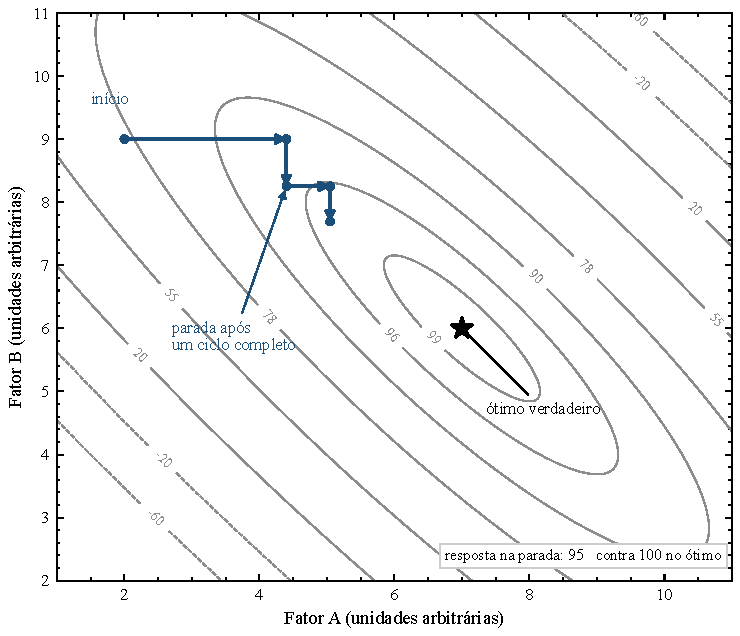
\includegraphics[width=0.80\linewidth]{../figuras/out/c1-um-fator-por-vez}
  \caption{Busca por otimização de um fator de cada vez sobre uma superfície
    de resposta sintética com interação acentuada entre os dois fatores. A
    trajetória alterna a otimização de cada fator com o outro mantido fixo
    e estaciona antes de alcançar o ótimo verdadeiro, marcado pela estrela,
    presa pela mesma interação que a geraria se fosse reconhecida.}
  \label{fig:ofat}
\end{figure}

A trajetória da Figura~\ref{fig:ofat} converge para um ponto estável, porém
distante do ótimo verdadeiro: o procedimento não tem como escapar dele, já
que cada movimento unidimensional o encontra como um máximo local ao longo
daquele corte. O planejamento fatorial evita essa armadilha por construir,
desde o primeiro ensaio, combinações que cobrem simultaneamente os níveis de
todos os fatores, tornando a interação mensurável em vez de invisível.

\begin{aplicacao}{Interação real medida num planejamento fatorial}
  No planejamento $2^{3}$ de temperatura, catalisador e concentração
  (Peixoto, Capítulo 3, páginas 18 a 26), o efeito de interação entre
  temperatura e catalisador foi estimado em
  $\efeito{T\cdot Cat} = \num{-8.625}$, valor comparável em módulo aos
  próprios efeitos principais de catalisador, $\num{-13.875}$, e de
  concentração, $\num{8.875}$. Um experimentador que tivesse fixado o
  catalisador no nível B antes de variar a temperatura, prática comum na
  otimização de um fator por vez, teria encontrado um ganho de rendimento
  com a temperatura muito menor do que o observado no nível A, e poderia
  concluir, erradamente, que a temperatura pouco importa. A leitura correta,
  obtida apenas porque o planejamento fatorial testa as quatro combinações
  de temperatura e catalisador, é que a concentração é relevante mas
  praticamente não interage com os demais fatores, podendo ser estudada em
  separado, ao passo que temperatura e catalisador precisam ser lidos em
  conjunto.
\end{aplicacao}

\section{Erros de medida}
\label{sec:erros-medida}

Toda medição se afasta, em algum grau, do valor que pretende representar. A
literatura de metrologia e de planejamento de experimentos distingue três
categorias desse afastamento, cada uma exigindo uma resposta diferente do
experimentador.

O erro grosseiro resulta de uma falha identificável e pontual: leitura
trocada, amostra contaminada, equipamento usado fora da especificação numa
única execução. Sua marca é ser um evento isolado, e o tratamento correto é
identificá-lo e excluir a observação afetada, nunca absorvê-la na análise
como se fosse variação normal. O erro sistemático desloca as medições
sempre na mesma direção e pela mesma magnitude, por uma causa que persiste
enquanto não for corrigida, como um instrumento descalibrado ou um
procedimento que favorece um resultado. Sua marca é o viés constante, e
nenhuma quantidade de repetição o revela, porque repetir o mesmo
procedimento enviesado reproduz o mesmo viés. O erro aleatório é a
variação residual que persiste mesmo quando nenhuma causa identificável está
presente, originada de fontes numerosas e pequenas que se somam de forma
imprevisível. Sua marca é a dispersão em torno de um valor central, e é o
único dos três que a réplica ataca diretamente, como a Seção~\ref{sec:erro-laboratorio}
demonstra.

\begin{aplicacao}{Dispersão aleatória em torno de uma especificação}
  A Figura~\ref{fig:dispersao} apresenta vinte medições de velocidade de
  boca de um mesmo lote de munição, comparadas à especificação de projeto
  de \qty{850}{\meter\per\second}.

  \begin{figure}[H]
    \centering
    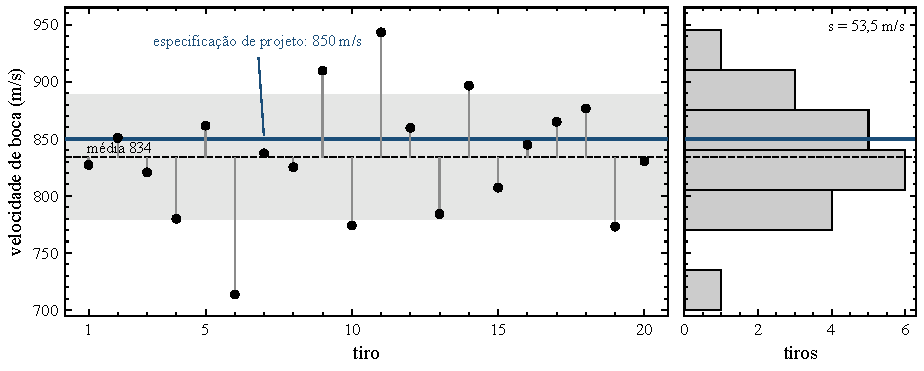
\includegraphics[width=\linewidth]{../figuras/out/c1-dispersao-20-medidas}
    \caption{Vinte medições de velocidade de boca, na ordem de disparo, e o
      histograma da mesma amostra à direita. A faixa sombreada indica um
      desvio-padrão em torno da média amostral, e a linha de apoio marca a
      especificação de projeto de \qty{850}{\meter\per\second} (fonte:
      Peixoto, Capítulos 1 e 2, página 10).}
    \label{fig:dispersao}
  \end{figure}

  A média amostral das vinte medições é \qty{834.0}{\meter\per\second}, com
  desvio-padrão de \qty{53.5}{\meter\per\second}; doze das vinte medições
  ficam abaixo da especificação e oito acima, sem qualquer tendência
  direcional visível na ordem de disparo. Esse padrão, disperso em torno de
  uma média estável e sem deriva sistemática, é a assinatura do erro
  aleatório: nenhum disparo isolado precisa ser descartado, e nenhum viés
  precisa ser corrigido, mas a variação é grande o bastante para que uma
  única medição não sirva de base para qualquer conclusão sobre o lote.
\end{aplicacao}

\section{O erro experimental no laboratório de materiais}
\label{sec:erro-laboratorio}

A distinção entre erro aleatório e erro sistemático parece abstrata até ser
confrontada com a rotina de um laboratório de materiais. Nessa rotina, cada
corpo de prova percorre um caminho longo, moldagem, cura, armazenamento,
ensaio, e cada etapa desse caminho é uma oportunidade para que um dos três
tipos de erro se manifeste. O que a réplica genuína oferece diante dessa
variação é uma redução previsível da incerteza sobre a média: se a
variância de uma medição individual é $\sigma^{2}$, a variância da média de
$N$ réplicas independentes é dada pela Equação~\eqref{eq:var-media}.

\begin{equation}
  \mathrm{Var}(\bar{x}) = \frac{\sigma^{2}}{N} .
  \label{eq:var-media}
\end{equation}

A Figura~\ref{fig:variancia} apresenta essa relação em função do número de
réplicas.

\begin{figure}[H]
  \centering
  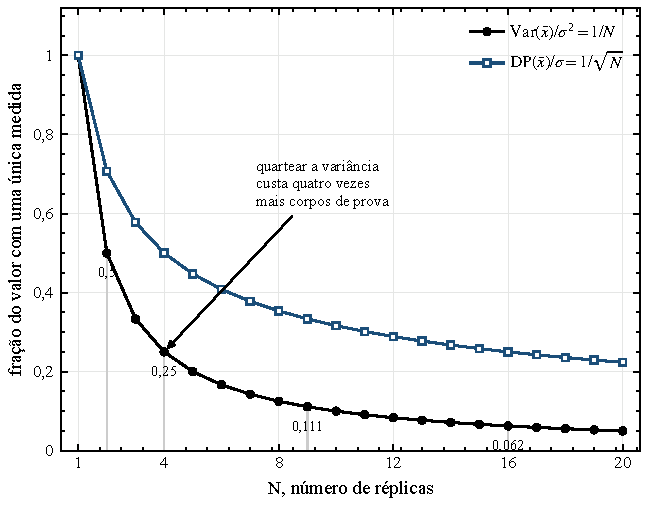
\includegraphics[width=0.70\linewidth]{../figuras/out/c1-variancia-da-media}
  \caption{Razão entre a variância da média e a variância individual,
    $\mathrm{Var}(\bar{x})/\sigma^{2} = 1/N$, e a razão análoga para o
    desvio-padrão, $1/\sqrt{N}$, em função do número de réplicas $N$. O
    ganho por réplica adicional decresce rapidamente: quadruplicar o número
    de réplicas de quatro para dezesseis reduz a variância da média a um
    quarto do valor anterior, de $0,25\,\sigma^{2}$ para
    $0,0625\,\sigma^{2}$.}
  \label{fig:variancia}
\end{figure}

A Equação~\eqref{eq:var-media} e a Figura~\ref{fig:variancia} deixam claro
o alcance e o limite da réplica. Ela dilui o erro aleatório porque esse
erro, por definição, varia de execução para execução e se cancela em parte
quando as execuções são combinadas. Ela não faz nada contra o erro
sistemático, porque um viés constante afeta igualmente todas as réplicas e
permanece, inteiro, na média por maior que seja $N$. Contra o erro
sistemático a ferramenta é outra: eliminar a causa do viés quando ela é
conhecida, ou, quando não é, impedir que ela se confunda com um fator de
interesse por meio de aleatorização e blocagem, temas das
Seções~\ref{sec:aleatorizacao} e \ref{sec:blocagem}.

\begin{aplicacao}{Classificação de desvios num laboratório de solo-fibra-cimento}
  Quatro situações, todas ocorridas na preparação de corpos de prova de
  solo, fibra vegetal amazônica e cimento, ilustram a taxonomia da
  Seção~\ref{sec:erros-medida} aplicada a um caso concreto. A
  Tabela~\ref{tab:classificacao-erros} classifica cada uma e indica o que
  ela exige da análise.

  \begin{table}[H]
    \centering
    \caption{Classificação de quatro desvios observados na preparação de
      corpos de prova, segundo a taxonomia de erro grosseiro, sistemático e
      aleatório.}
    \label{tab:classificacao-erros}
    \begin{tabular}{p{0.30\linewidth} p{0.16\linewidth} p{0.46\linewidth}}
      \toprule
      \textbf{Situação} & \textbf{Classificação} & \textbf{O que a análise exige} \\
      \midrule
      Um corpo de prova permaneceu na estufa muito além do tempo
      prescrito. &
      Grosseiro &
      Identificar e excluir o corpo de prova afetado; repeti-lo se o
      material disponível permitir. Réplica adicional não corrige uma
      leitura já invalidada. \\
      \addlinespace
      Um corpo de prova estava na estufa durante uma queda de energia. &
      Grosseiro &
      Mesmo tratamento do caso anterior: o ciclo de secagem foi
      interrompido de forma imprevisível e o resultado não representa a
      condição pretendida, devendo ser descartado e documentado. \\
      \addlinespace
      Um lote de corpos de prova ficou armazenado em ambiente mais úmido
      antes da moldagem. &
      Sistemático &
      Não se corrige por réplica, porque o viés atinge igualmente todas as
      repetições desse lote. Exige aleatorizar a distribuição dos lotes
      entre as condições do experimento ou tratar o lote como bloco. \\
      \addlinespace
      Houve segregação da fibra durante o quarteamento do material. &
      Sistemático &
      Um procedimento de quarteamento tendencioso desloca o teor de fibra
      efetivo na mesma direção em todas as alíquotas que dele derivam.
      Exige revisão do procedimento de quarteamento e aleatorização de qual
      alíquota alimenta qual corpo de prova, não apenas mais repetições. \\
      \bottomrule
    \end{tabular}
  \end{table}

  Nenhum dos quatro casos é um exemplo de erro aleatório, o que é
  proposital: são justamente os casos em que aumentar o número de réplicas,
  sozinho, não resolveria nada. Os dois primeiros exigem um critério de
  exclusão e, quando possível, a repetição do corpo de prova; os dois
  últimos exigem aleatorização ou blocagem, não uma média mais bem estimada
  sobre dados que carregam o mesmo viés.
\end{aplicacao}

\section{Réplicas}
\label{sec:replicas}

A réplica genuína é a repetição completa e independente de uma mesma
condição experimental, do início ao fim do procedimento, e não a medição
repetida de uma única execução. Essa distinção é decisiva: medir duas vezes
a mesma amostra estima o erro do instrumento de leitura, ao passo que
preparar duas amostras independentes sob a mesma condição estima o erro
experimental completo, que inclui a preparação, a montagem e a medição.
Tratar a segunda coisa como se fosse a primeira produz uma estimativa de
erro artificialmente pequena e infla a aparência de significância dos
efeitos, um dos itens listados entre as condições que invalidam uma
análise.

A réplica é a única fonte de erro puro: a variabilidade observada entre
execuções nominalmente idênticas, isto é, entre réplicas de um mesmo
tratamento. Sem essa estimativa, não existe padrão contra o qual comparar a
falta de ajuste de um modelo, e o teste correspondente, apresentado no
Caderno~3, simplesmente não pode ser calculado. Réplica insuficiente não é
apenas um problema de precisão: é a ausência de um instrumento de
diagnóstico inteiro.

Esse benefício tem custo. Replicar integralmente todas as condições de um
planejamento consome, segundo estimativa reportada em material de apoio da
disciplina, algo em torno de setenta por cento do esforço experimental
total, o que explica por que a decisão de quantas réplicas incluir, e onde
incluí-las, é tratada com tanto cuidado nos cadernos seguintes.

O custo cresce de forma linear com o número de réplicas, mas o benefício,
pela Equação~\eqref{eq:var-media} da Seção~\ref{sec:erro-laboratorio}, cresce
apenas com a raiz quadrada desse número. Passar de duas para quatro réplicas
reduz o desvio-padrão da média por um fator de $\sqrt{2}$, uma melhora
substancial pelo custo de dobrar o esforço; passar de dezesseis para trinta
e duas réplicas reduz o mesmo desvio-padrão pelo mesmo fator de $\sqrt{2}$,
mas ao custo de seis vezes mais ensaios do que o par inicial. Esse retorno
decrescente é o motivo pelo qual, diante de material escasso, discutido na
Seção~\ref{sec:material-escasso}, a resposta correta raramente é replicar
mais: costuma ser concentrar as poucas réplicas disponíveis exatamente nos
pontos em que a estimativa de erro puro é indispensável, e não distribuí-las
igualmente por toda a matriz de ensaios.

\begin{aplicacao}{Erro puro a partir de réplicas reais}
  A Tabela~\ref{tab:variancias-catalisador} retoma o experimento de
  rendimento da Seção~\ref{sec:fator-nivel} e mostra a variância amostral
  calculada dentro de cada par de réplicas.

  \begin{table}[H]
    \centering
    \caption{Variância amostral em cada uma das quatro condições do
      planejamento $2^{2}$ de rendimento, com duas réplicas por condição.}
    \label{tab:variancias-catalisador}
    \begin{tabular}{c S[table-format=3.0] c S[table-format=1.0]}
      \toprule
      {Ensaio} & {T (\si{\kelvin})} & {Catalisador} & {Variância} \\
      \midrule
      1 & 313 & A & 8 \\
      2 & 333 & A & 8 \\
      3 & 313 & B & 2 \\
      4 & 333 & B & 8 \\
      \bottomrule
    \end{tabular}
  \end{table}

  Cada condição contribui um grau de liberdade para a estimativa de erro
  puro, porque cada par de réplicas tem $n_{i} - 1 = 1$ grau de liberdade.
  Combinando as quatro variâncias em partes iguais obtém-se a variância
  combinada $S^{2} = (8 + 8 + 2 + 8)/4 = \num{6.5}$, com quatro graus de
  liberdade, que é exatamente o erro puro do experimento. É esse número,
  e não uma suposição teórica sobre o instrumento, que sustenta o
  julgamento de quais efeitos, apresentados no Caderno~2, se distinguem do
  ruído experimental (fonte: Peixoto, Capítulo 3, páginas 2 a 9).
\end{aplicacao}

\section{Aleatorização}
\label{sec:aleatorizacao}

Aleatorizar significa sortear a ordem em que as combinações de níveis serão
executadas, em vez de segui-las na sequência em que aparecem na tabela do
planejamento. A razão é protegê-lo contra qualquer tendência que se
desenvolva ao longo do tempo de execução, como o aquecimento gradual de um
equipamento, o desgaste de uma ferramenta de corte ou a variação de umidade
do ar ao longo de um dia de ensaios. Se a ordem de execução seguisse a
ordem da tabela, uma tendência temporal desse tipo se confundiria com o
próprio efeito de um fator, porque ambos cresceriam ou decresceriam
juntos ao longo da sequência. O procedimento concreto é simples: numerar as
combinações previstas, sortear uma permutação dessa numeração por meio de
um gerador de números aleatórios ou de um sorteio físico equivalente, e
executar os ensaios na ordem sorteada, documentando-a antes de começar.

\begin{aplicacao}{Ordem sorteada de execução num planejamento real}
  A Tabela~\ref{tab:aleatorizacao} reproduz a ordem padrão e a ordem
  efetivamente sorteada de um planejamento fatorial $2^{2}$ com duas
  réplicas, empregado num ensaio de deformação permanente com os fatores
  identificados na fonte como \emph{cond} e \emph{par}.

  \begin{table}[H]
    \centering
    \caption{Ordem padrão das oito combinações de um planejamento $2^{2}$
      com duas réplicas e a ordem efetivamente sorteada para a execução.}
    \label{tab:aleatorizacao}
    \begin{tabular}{c c c c}
      \toprule
      {Ordem padrão} & {cond} & {par} & {Ordem sorteada} \\
      \midrule
      1 & $-1$ (18) & $-1$ (70,70)  & 2 \\
      2 & $+1$ (19) & $-1$ (70,70)  & 1 \\
      3 & $+1$ (19) & $+1$ (210,70) & 4 \\
      4 & $-1$ (18) & $+1$ (210,70) & 3 \\
      5 & $-1$ (18) & $-1$ (70,70)  & 5 \\
      6 & $+1$ (19) & $-1$ (70,70)  & 6 \\
      7 & $+1$ (19) & $+1$ (210,70) & 8 \\
      8 & $-1$ (18) & $+1$ (210,70) & 7 \\
      \bottomrule
    \end{tabular}
  \end{table}

  A ordem padrão, mostrada na primeira coluna, é apenas uma listagem
  sistemática das combinações de níveis, conveniente para conferir que
  nenhuma delas foi esquecida. A ordem sorteada, mostrada na última coluna,
  é a que de fato guiou a execução no laboratório: a terceira combinação
  padrão só foi executada na quarta posição real, e assim por diante. Um
  eventual efeito de deriva ao longo do dia de ensaio, se existisse,
  afetaria posições da ordem sorteada, não condições específicas de
  \emph{cond} ou \emph{par}, e por isso não poderia ser confundido com o
  efeito desses fatores (fonte: painel do software Statistica reproduzido
  na disciplina, conferido pelo motor computacional do programa que
  acompanha estes cadernos).
\end{aplicacao}

\section{Blocagem}
\label{sec:blocagem}

Quando uma fonte de variação sistemática é conhecida de antemão, mas não é
o objeto de interesse do experimento, ela deve ser tratada como bloco: os
ensaios são agrupados de modo que cada bloco contenha uma repetição
completa das condições que se deseja comparar, e a comparação é feita
dentro de cada bloco, não entre blocos. Isso remove a variação entre blocos
da estimativa de erro, em vez de deixá-la inflar a dispersão total e
mascarar a diferença de interesse.

O exemplo mais direto dessa ideia é o teste pareado. Ao comparar duas
condições usando a mesma unidade experimental sob as duas condições, ou
unidades emparelhadas por uma característica relevante, o intervalo de
confiança para a diferença é constru\'ido sobre as diferenças individuais,
$d_{i}$, conforme a Equação~\eqref{eq:intervalo-pareado}, em vez de sobre a
diferença entre médias de dois grupos independentes, conforme a
Equação~\eqref{eq:intervalo-nao-pareado}.

\begin{equation}
  \bar{d} \pm t^{*}_{\nu} \cdot \frac{S_{d}}{\sqrt{n}} ,
  \qquad \nu = n - 1 .
  \label{eq:intervalo-pareado}
\end{equation}

\begin{equation}
  (\bar{x}_{1} - \bar{x}_{2}) \pm t^{*}_{\nu} \cdot S_{p}\sqrt{\frac{2}{n}} ,
  \qquad \nu = 2(n-1) .
  \label{eq:intervalo-nao-pareado}
\end{equation}

A diferença entre as duas equações não é apenas de forma. Ao emparelhar as
observações, a Equação~\eqref{eq:intervalo-pareado} usa o desvio-padrão das
diferenças, $S_{d}$, que exclui a variação entre pares por construção. A
Equação~\eqref{eq:intervalo-nao-pareado} usa o desvio-padrão combinado dos
dois grupos, $S_{p}$, que inclui essa variação inteira. Quando ela é grande
frente à diferença de interesse, a segunda equação produz um intervalo
muito mais largo do que a primeira, para os mesmos dez números.

\begin{aplicacao}{Os cinco pares arma-radar}
  Cinco conjuntos de arma e radar tiveram sua velocidade de boca medida com
  munições de cinco fabricantes diferentes, um par de medições por
  fabricante. A Tabela~\ref{tab:armaradar-dados} apresenta os dez valores.

  \begin{table}[H]
    \centering
    \caption{Velocidade de boca, em \unit{\meter\per\second}, de dois
      conjuntos arma-radar, medida com munição de cinco fabricantes.}
    \label{tab:armaradar-dados}
    \begin{tabular}{c S[table-format=3.0] S[table-format=3.0] S[table-format=-2.0]}
      \toprule
      {Fabricante} & {Conjunto 1} & {Conjunto 2} & {Diferença} \\
      \midrule
      1 & 377 & 362 & 15 \\
      2 & 385 & 369 & 16 \\
      3 & 407 & 410 & -3 \\
      4 & 483 & 470 & 13 \\
      5 & 505 & 489 & 16 \\
      \bottomrule
    \end{tabular}
  \end{table}

  A média do conjunto 1 é \qty{431.4}{\meter\per\second} e a do conjunto 2 é
  \qty{420.0}{\meter\per\second}, uma diferença de
  \qty{11.4}{\meter\per\second}. A Tabela~\ref{tab:armaradar-resultado}
  aplica as Equações~\eqref{eq:intervalo-pareado} e
  \eqref{eq:intervalo-nao-pareado} aos mesmos dez números.

  \begin{table}[H]
    \centering
    \caption{Intervalo de \qty{95}{\percent} de confiança para a diferença
      entre os dois conjuntos arma-radar, com e sem reconhecer o fabricante
      como bloco.}
    \label{tab:armaradar-resultado}
    \begin{tabular}{l c c l}
      \toprule
      \textbf{Análise} & $t^{*}$ & \textbf{Semi-amplitude} & \textbf{Intervalo} \\
      \midrule
      Sem blocagem (2 amostras, 8 GL) & 2,306 & \qty{84.91}{\meter\per\second} & $11,4 \pm 84,91$, contém zero \\
      Com blocagem (pareado, 4 GL) & 2,776 & \qty{10.11}{\meter\per\second} & $11,4 \pm 10,11$, não contém zero \\
      \bottomrule
    \end{tabular}
  \end{table}

  A Figura~\ref{fig:blocagem-intervalo} apresenta a dispersão das dez
  medições originais por fabricante e os dois intervalos de confiança
  contrapostos, sem e com o reconhecimento do bloco.

  \begin{figure}[H]
    \centering
    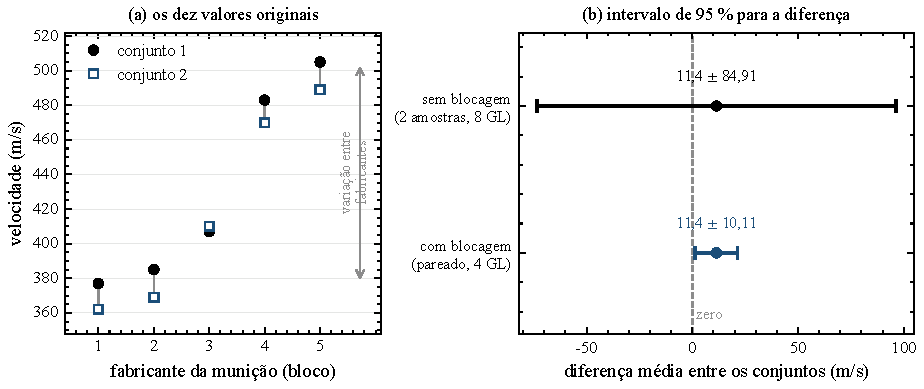
\includegraphics[width=0.65\linewidth]{../figuras/out/c1-blocagem-intervalo}
    \caption{Os dez valores de velocidade de boca dos cinco pares
      arma-radar, agrupados por fabricante, e os intervalos de
      \qty{95}{\percent} de confiança para a diferença entre os dois
      conjuntos, sem e com o reconhecimento do fabricante como bloco: o
      primeiro intervalo contém zero, o segundo não (fonte: Peixoto,
      Capítulos 1 e 2, páginas 47 a 53).}
    \label{fig:blocagem-intervalo}
  \end{figure}

  Os mesmos dez números levam a conclusões opostas conforme o fabricante
  seja ou não reconhecido como bloco. Sem blocagem, a variabilidade entre
  fabricantes, que vai de \qty{377}{\meter\per\second} a
  \qty{505}{\meter\per\second}, é tratada como se fosse ruído do
  experimento e engole a diferença de \qty{11.4}{\meter\per\second} entre
  os conjuntos, produzindo um intervalo que contém zero. Com blocagem, essa
  mesma variabilidade é removida da comparação, o intervalo se estreita em
  cerca de oito vezes, e a diferença se revela estatisticamente
  significativa (fonte: Peixoto, Capítulos 1 e 2, páginas 47 a 53). Vale
  registrar que a publicação original desse exemplo traz, na página 52, um
  episódio do próprio tema deste caderno: o intervalo sem blocagem está
  impresso como $11,4 \pm 84,1$, quando o recálculo a partir dos mesmos dez
  números fornece $84,91$. A conclusão não muda, porque o intervalo contém
  zero nos dois casos, mas o episódio é um lembrete de que a conferência
  independente dos números é parte do próprio método, não uma formalidade.
\end{aplicacao}

\section{Material escasso}
\label{sec:material-escasso}

Até aqui, o número de ensaios foi tratado como uma escolha do
experimentador, limitada apenas pelo tempo e pelo orçamento financeiro. Há
uma restrição adicional, comum em pesquisa com materiais não convencionais,
que precisa entrar no planejamento desde o primeiro momento: a quantidade
de matéria-prima disponível. No estudo de solo, fibra e cimento que
acompanha este caderno, a fibra vegetal empregada é de origem amazônica e
foi trazida de Manaus por via aérea em quantidade finita e conhecida desde
o início. Essa quantidade, e não uma preferência metodológica, é o que
determina quantos corpos de prova podem ser moldados ao longo de toda a
pesquisa. O número de ensaios deixa de ser uma variável de projeto e passa
a ser uma restrição de projeto, na mesma categoria de um prazo fixo ou de
um equipamento indisponível.

Essa restrição muda a pergunta que o planejamento precisa responder. Em vez
de perguntar quantos ensaios seriam desejáveis para estimar todos os
efeitos e interações com a precisão que a teoria recomenda, o
experimentador precisa perguntar quantos fatores podem ser investigados com
o número de corpos de prova que o material disponível permite moldar, e o
que sacrificar quando os dois números não coincidem. O Caderno~5 desenvolve
essa questão em detalhe e apresenta duas saídas complementares para o
mesmo problema: o planejamento fatorial fracionado, que reduz o número de
ensaios aceitando confundir interações de ordem alta entre si, e a
triagem por planos saturados, que investiga o maior número possível de
fatores no menor número possível de ensaios, ao custo de uma confiança
menor sobre cada fator individual.

A escolha entre essas duas saídas depende do estágio em que a pesquisa se
encontra, não de uma preferência fixa por um tipo de arranjo. No início de
um programa experimental, quando a lista de fatores candidatos ainda é
longa e pouco se sabe sobre quais deles de fato importam, a triagem por um
plano saturado é a escolha racional: descartar rapidamente os fatores
irrelevantes libera o material restante para investigar com profundidade
os poucos que sobrevivem à triagem. Mais adiante, quando o número de
fatores relevantes já foi reduzido a dois ou três, o mesmo orçamento de
material rende mais informação se investido num planejamento fatorial
completo, ou mesmo numa composição central, sobre esse conjunto reduzido,
do que se ainda fosse gasto tentando confirmar fatores que a triagem já
descartou. Decidir errado essa sequência, otimizando cedo demais um
conjunto de fatores ainda não filtrado, é uma forma comum de desperdiçar
justamente o material mais escasso.

\begin{aplicacao}{A economia de um planejamento fracionado}
  A Tabela~\ref{tab:orcamento-material} contrasta o número de ensaios que um
  planejamento fatorial completo exigiria para sete fatores em dois níveis
  com o número efetivamente empregado num planejamento fracionado saturado
  para o mesmo escopo.

  \begin{table}[H]
    \centering
    \caption{Número de ensaios para investigar sete fatores em dois
      níveis, com e sem fracionamento.}
    \label{tab:orcamento-material}
    \begin{tabular}{l S[table-format=3.0]}
      \toprule
      \textbf{Planejamento} & {Ensaios} \\
      \midrule
      Fatorial completo $2^{7}$ & 128 \\
      Fatorial fracionado saturado $2^{7-4}_{\mathrm{III}}$ & 8 \\
      \bottomrule
    \end{tabular}
  \end{table}

  O planejamento fracionado saturado, construído a partir de um fatorial
  completo de três fatores com quatro colunas adicionais geradas por
  produtos entre elas, ocupa dezesseis vezes menos ensaios que o fatorial
  completo equivalente, ao custo de confundir cada efeito principal com um
  conjunto de interações que a análise não consegue separar sozinha (fonte:
  Peixoto, Capítulo 4, páginas 34 a 42). Para um orçamento de material que
  permita moldar apenas alguns corpos de prova, essa é frequentemente a
  única forma de investigar mais de dois ou três fatores sem esgotar o
  material antes de qualquer conclusão ser possível. O Caderno~5 mostra
  como decidir, caso a caso, se esse custo compensa.
\end{aplicacao}

\section{Exemplo de aplicação}
\label{sec:exemplo-final}

Fecha-se o caderno com o planejamento de um estudo real, o mesmo que
fornece o pano de fundo dos exemplos das Seções~\ref{sec:erro-laboratorio}
e \ref{sec:material-escasso}: a caracterização de um compósito de solo,
fibra vegetal amazônica e cimento, destinado a aplicações de pavimentação
ou de contenção geotécnica.

A revisão bibliográfica que precede um estudo desse tipo levanta uma lista
longa de parâmetros candidatos a fator: o teor de cimento, o teor de fibra,
o tipo e a procedência da fibra, o comprimento das fibras incorporadas, o
teor de umidade de compactação, a energia de compactação, o tempo e a
condição de cura, e a idade do corpo de prova no momento do ensaio. Testar
todos esses parâmetros simultaneamente exigiria um número de ensaios muito
além do que o material disponível permite, conforme discutido na
Seção~\ref{sec:material-escasso}, de modo que a lista precisa ser reduzida
antes que qualquer matriz de ensaios seja desenhada.

A redução segue o mesmo raciocínio da Seção~\ref{sec:hipotese}: um
parâmetro só permanece como fator variável se a hipótese de pesquisa e a
literatura correlata indicarem que ele influencia a resposta de interesse
de forma ainda não bem quantificada para o material em estudo. Os demais
parâmetros não desaparecem do planejamento, eles são fixados em um valor
único, escolhido pela prática consolidada na literatura ou pela
disponibilidade real de material, e passam a integrar a descrição do
experimento em vez de sua matriz de ensaios. O tipo de fibra é o exemplo
mais direto dessa fixação: havendo apenas um lote da fibra amazônica
disponível, comparar tipos de fibra deixa de ser uma pergunta que este
estudo pode responder, e o tipo passa de fator candidato a característica
fixa do material. A energia de compactação e o teor de umidade de
compactação, por sua vez, são fixados no valor de referência estabelecido
pela norma de ensaio adotada, por já estarem bem documentados na literatura
de solo-cimento.

O que resta depois dessa redução são os fatores quantitativos cuja faixa de
variação a literatura ainda não cobre para o par solo-fibra em estudo: o
teor de cimento, o teor de fibra, e a idade do corpo de prova no momento do
ensaio de resistência, esta última incluída porque a evolução da
resistência ao longo da cura é, ela própria, parte da pergunta de pesquisa.
A resposta escolhida é a resistência à compressão simples, por ser a
grandeza mecânica de referência na caracterização desse tipo de compósito e
por se relacionar diretamente com a aplicação em pavimentação pretendida.

Esse é o padrão que percorre todo o caderno, aplicado de uma só vez: a
hipótese de pesquisa e a revisão bibliográfica selecionam os fatores
(Seções~\ref{sec:fator-nivel} e \ref{sec:hipotese}); o planejamento
fatorial, e não a variação de um fator por vez, é o que permite enxergar
eventuais interações entre teor de cimento e teor de fibra
(Seção~\ref{sec:ofat}); a quantidade de fibra disponível limita o número de
corpos de prova e orienta a escolha entre um planejamento completo e um
fracionado (Seção~\ref{sec:material-escasso}); e réplicas, aleatorização e
blocagem, quando a moldagem se estender por mais de um dia ou empregar mais
de um lote de material, protegem a análise final contra exatamente os tipos
de desvio catalogados na Seção~\ref{sec:erro-laboratorio}. O Caderno~2
retoma esse planejamento no ponto em que este caderno o deixa, ao formalizar
a matriz de ensaios de um planejamento fatorial em dois níveis.

\paginadireitos

\end{document}
